% Created by tikzDevice version 0.12.3.1 on 2022-09-02 16:30:05
% !TEX encoding = UTF-8 Unicode
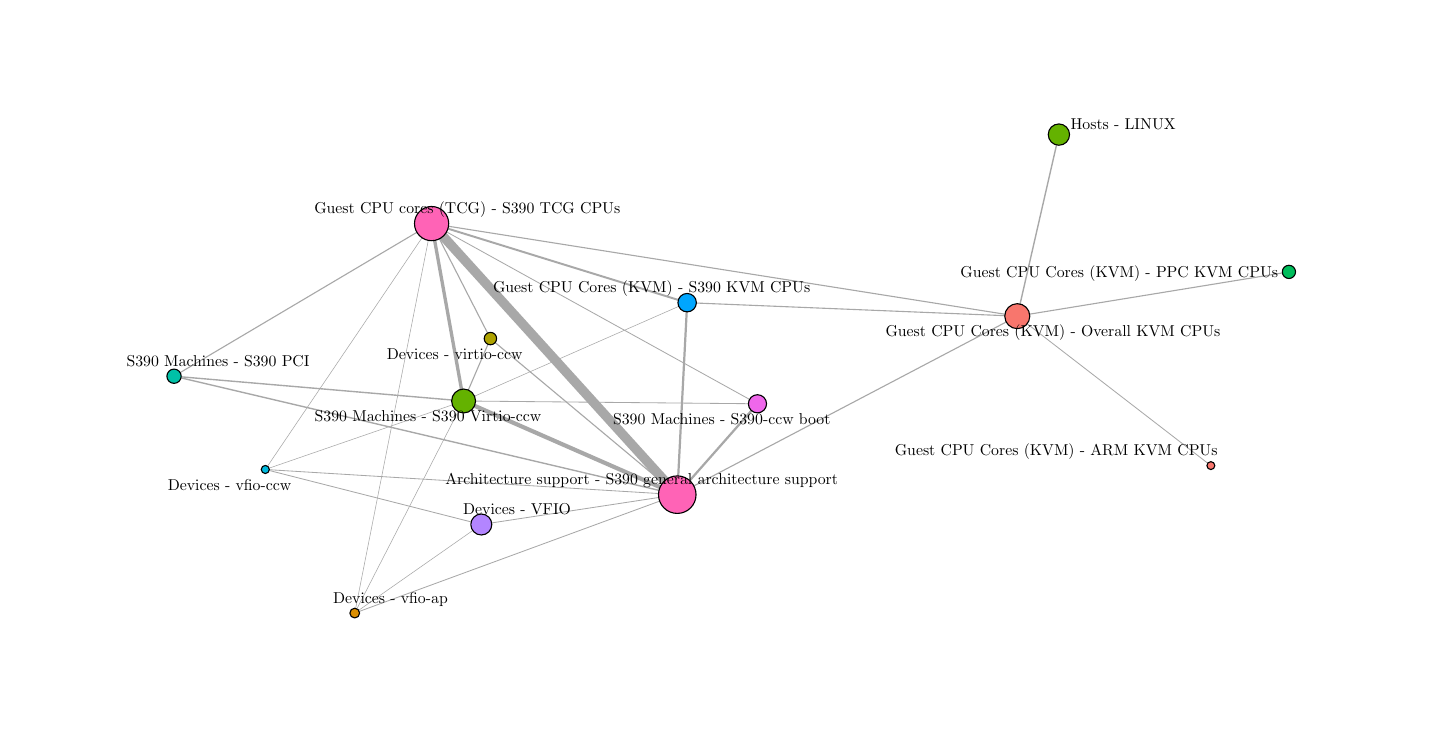
\begin{tikzpicture}[x=1pt,y=1pt]
\definecolor{fillColor}{RGB}{255,255,255}
\path[use as bounding box,fill=fillColor,fill opacity=0.00] (0,0) rectangle (505.89,252.94);
\begin{scope}
\path[clip] (  0.00,  0.00) rectangle (505.89,252.94);
\definecolor{fillColor}{RGB}{255,255,255}

\path[fill=fillColor] (  0.00,  0.00) rectangle (505.89,252.94);
\end{scope}
\begin{scope}
\path[clip] ( 32.75, 32.75) rectangle (475.89,222.94);
\definecolor{drawColor}{gray}{0.66}

\path[draw=drawColor,line width= 0.3pt,line join=round] (234.73, 84.19) -- (163.92, 73.41);

\path[draw=drawColor,line width= 0.3pt,line join=round] (234.73, 84.19) -- (118.18, 41.40);

\path[draw=drawColor,line width= 0.3pt,line join=round] (234.73, 84.19) -- ( 85.86, 93.29);

\path[draw=drawColor,line width= 0.4pt,line join=round] (234.73, 84.19) -- (167.21,140.59);

\path[draw=drawColor,line width= 0.4pt,line join=round] (234.73, 84.19) -- (357.59,148.69);

\path[draw=drawColor,line width= 0.8pt,line join=round] (234.73, 84.19) -- (238.30,153.57);

\path[draw=drawColor,line width= 3.4pt,line join=round] (234.73, 84.19) -- (145.96,182.14);

\path[draw=drawColor,line width= 0.5pt,line join=round] (234.73, 84.19) -- ( 52.89,126.99);

\path[draw=drawColor,line width= 1.5pt,line join=round] (234.73, 84.19) -- (157.52,118.04);

\path[draw=drawColor,line width= 0.8pt,line join=round] (234.73, 84.19) -- (263.71,117.03);

\path[draw=drawColor,line width= 0.2pt,line join=round] (163.92, 73.41) -- (118.18, 41.40);

\path[draw=drawColor,line width= 0.3pt,line join=round] (163.92, 73.41) -- ( 85.86, 93.29);

\path[draw=drawColor,line width= 0.2pt,line join=round] (118.18, 41.40) -- (145.96,182.14);

\path[draw=drawColor,line width= 0.2pt,line join=round] (118.18, 41.40) -- (157.52,118.04);

\path[draw=drawColor,line width= 0.2pt,line join=round] ( 85.86, 93.29) -- (145.96,182.14);

\path[draw=drawColor,line width= 0.2pt,line join=round] ( 85.86, 93.29) -- (157.52,118.04);

\path[draw=drawColor,line width= 0.4pt,line join=round] (167.21,140.59) -- (145.96,182.14);

\path[draw=drawColor,line width= 0.4pt,line join=round] (167.21,140.59) -- (157.52,118.04);

\path[draw=drawColor,line width= 0.3pt,line join=round] (427.54, 94.69) -- (357.59,148.69);

\path[draw=drawColor,line width= 0.4pt,line join=round] (357.59,148.69) -- (455.75,164.69);

\path[draw=drawColor,line width= 0.4pt,line join=round] (357.59,148.69) -- (238.30,153.57);

\path[draw=drawColor,line width= 0.4pt,line join=round] (357.59,148.69) -- (145.96,182.14);

\path[draw=drawColor,line width= 0.5pt,line join=round] (357.59,148.69) -- (372.63,214.30);

\path[draw=drawColor,line width= 0.7pt,line join=round] (238.30,153.57) -- (145.96,182.14);

\path[draw=drawColor,line width= 0.2pt,line join=round] (238.30,153.57) -- (157.52,118.04);

\path[draw=drawColor,line width= 0.4pt,line join=round] (145.96,182.14) -- ( 52.89,126.99);

\path[draw=drawColor,line width= 1.2pt,line join=round] (145.96,182.14) -- (157.52,118.04);

\path[draw=drawColor,line width= 0.3pt,line join=round] (145.96,182.14) -- (263.71,117.03);

\path[draw=drawColor,line width= 0.5pt,line join=round] ( 52.89,126.99) -- (157.52,118.04);

\path[draw=drawColor,line width= 0.3pt,line join=round] (157.52,118.04) -- (263.71,117.03);
\definecolor{drawColor}{RGB}{0,0,0}
\definecolor{fillColor}{RGB}{255,99,182}

\path[draw=drawColor,line width= 0.4pt,line join=round,line cap=round,fill=fillColor] (234.73, 84.19) circle (  6.78);
\definecolor{fillColor}{RGB}{179,133,255}

\path[draw=drawColor,line width= 0.4pt,line join=round,line cap=round,fill=fillColor] (163.92, 73.41) circle (  3.79);
\definecolor{fillColor}{RGB}{219,142,0}

\path[draw=drawColor,line width= 0.4pt,line join=round,line cap=round,fill=fillColor] (118.18, 41.40) circle (  1.76);
\definecolor{fillColor}{RGB}{0,186,222}

\path[draw=drawColor,line width= 0.4pt,line join=round,line cap=round,fill=fillColor] ( 85.86, 93.29) circle (  1.46);
\definecolor{fillColor}{RGB}{174,162,0}

\path[draw=drawColor,line width= 0.4pt,line join=round,line cap=round,fill=fillColor] (167.21,140.59) circle (  2.24);
\definecolor{fillColor}{RGB}{248,118,109}

\path[draw=drawColor,line width= 0.4pt,line join=round,line cap=round,fill=fillColor] (427.54, 94.69) circle (  1.43);

\path[draw=drawColor,line width= 0.4pt,line join=round,line cap=round,fill=fillColor] (357.59,148.69) circle (  4.52);
\definecolor{fillColor}{RGB}{0,189,92}

\path[draw=drawColor,line width= 0.4pt,line join=round,line cap=round,fill=fillColor] (455.75,164.69) circle (  2.39);
\definecolor{fillColor}{RGB}{0,166,255}

\path[draw=drawColor,line width= 0.4pt,line join=round,line cap=round,fill=fillColor] (238.30,153.57) circle (  3.33);
\definecolor{fillColor}{RGB}{255,99,182}

\path[draw=drawColor,line width= 0.4pt,line join=round,line cap=round,fill=fillColor] (145.96,182.14) circle (  6.18);
\definecolor{fillColor}{RGB}{100,178,0}

\path[draw=drawColor,line width= 0.4pt,line join=round,line cap=round,fill=fillColor] (372.63,214.30) circle (  3.85);
\definecolor{fillColor}{RGB}{0,193,167}

\path[draw=drawColor,line width= 0.4pt,line join=round,line cap=round,fill=fillColor] ( 52.89,126.99) circle (  2.58);
\definecolor{fillColor}{RGB}{100,178,0}

\path[draw=drawColor,line width= 0.4pt,line join=round,line cap=round,fill=fillColor] (157.52,118.04) circle (  4.32);
\definecolor{fillColor}{RGB}{239,103,235}

\path[draw=drawColor,line width= 0.4pt,line join=round,line cap=round,fill=fillColor] (263.71,117.03) circle (  3.28);

\node[text=drawColor,anchor=base,inner sep=0pt, outer sep=0pt, scale=  0.57] at (221.89, 87.74) {Architecture support - S390 general architecture support};

\node[text=drawColor,anchor=base,inner sep=0pt, outer sep=0pt, scale=  0.57] at (176.84, 76.99) {Devices - VFIO};

\node[text=drawColor,anchor=base,inner sep=0pt, outer sep=0pt, scale=  0.57] at (131.09, 44.97) {Devices - vfio-ap};

\node[text=drawColor,anchor=base,inner sep=0pt, outer sep=0pt, scale=  0.57] at ( 72.95, 85.78) {Devices - vfio-ccw};

\node[text=drawColor,anchor=base,inner sep=0pt, outer sep=0pt, scale=  0.57] at (154.30,133.07) {Devices - virtio-ccw};

\node[text=drawColor,anchor=base,inner sep=0pt, outer sep=0pt, scale=  0.57] at (371.66, 98.22) {Guest CPU Cores (KVM) - ARM KVM CPUs};

\node[text=drawColor,anchor=base,inner sep=0pt, outer sep=0pt, scale=  0.57] at (370.47,141.22) {Guest CPU Cores (KVM) - Overall KVM CPUs};

\node[text=drawColor,anchor=base,inner sep=0pt, outer sep=0pt, scale=  0.57] at (394.46,162.73) {Guest CPU Cores (KVM) - PPC KVM CPUs};

\node[text=drawColor,anchor=base,inner sep=0pt, outer sep=0pt, scale=  0.57] at (225.47,157.14) {Guest CPU Cores (KVM) - S390 KVM CPUs};

\node[text=drawColor,anchor=base,inner sep=0pt, outer sep=0pt, scale=  0.57] at (158.85,185.71) {Guest CPU cores (TCG) - S390 TCG CPUs};

\node[text=drawColor,anchor=base,inner sep=0pt, outer sep=0pt, scale=  0.57] at (395.84,216.01) {Hosts - LINUX};

\node[text=drawColor,anchor=base,inner sep=0pt, outer sep=0pt, scale=  0.57] at ( 68.80,130.56) {S390 Machines - S390 PCI};

\node[text=drawColor,anchor=base,inner sep=0pt, outer sep=0pt, scale=  0.57] at (144.67,110.57) {S390 Machines - S390 Virtio-ccw};

\node[text=drawColor,anchor=base,inner sep=0pt, outer sep=0pt, scale=  0.57] at (250.82,109.52) {S390 Machines - S390-ccw boot};
\end{scope}
\end{tikzpicture}
